\documentclass[a4paper,10pt]{article}

\usepackage{amsmath}
\usepackage{amssymb}
\usepackage[usenames,dvipsnames]{color}
\usepackage{comment}
\usepackage[utf8]{inputenc}
\usepackage{listings}
\usepackage[pdfborder={0 0 0}]{hyperref}
\usepackage{spverbatim}
\usepackage{booktabs}
\usepackage{graphicx}

\definecolor{OliveGreen}{cmyk}{0.64,0,0.95,0.40}
\definecolor{Gray}{gray}{0.5}

\lstset{
    language=C,
    basicstyle=\ttfamily,
    keywordstyle=\color{OliveGreen},
    commentstyle=\color{Gray},
    captionpos=b,
    breaklines=true,
    breakatwhitespace=false,
    showspaces=false,
    showtabs=false,
    numbers=left,
}

\title{VU High Performance Computing \\
       SS 2013 \\
       Block 1: Memory Hierarchy \\
       lru-misses}
\author{Jakob Gruber, 0203440}

\begin{document}

\maketitle

\tableofcontents

\pagebreak

\section{Introduction} \label{section:introduction}

In this exercise, we implemented an algorithm to efficiently calculate stack distances
for a memory trace. These were then used to output the number of cache misses incurred by the
LRU eviction policy for stack sizes $2^i, i \in [0, 64]$.

Caches play a critical part in the performance of a computer program.
They are designed to exploit common characteristics of programs such as
spatial and temporal locality to avoid cache misses (which require
loading data from slower memory sections). This can be achieved by
so-called eviction policies, which decide which cache items are
to be discarded when the cache runs out of space.

To optimally exploit temporal locality, the policy would need to evict
the item which will not be needed for the longest time in the future. To do this, the algorithm would need know the future, which we have not been able to accomplish yet.

A good and practical solution is the \emph{Least Recently Used} (LRU)
policy, which simply evicts the item which has not been referenced for the largest amount of time. This exercise examines the behavior of the LRU algorithm for different stack sizes.

A memory trace contains all memory references incurred by the execution
of a program in their original order. We can simulate an LRU cache simply by iterating through the references and maintaining a stack as follows: 

\begin{itemize}
\item If the current address $a$ is not in the stack, it is placed on top.      and its stack distance $d$ is defined as $\infty$.
\item If it is in the stack, $d$ is defined as the position of $a$ within the stack.
      $a$ is then removed and subsequently placed on top.
\end{itemize}

A stack distance $d$ which is equal or greater to the cache size results
in a cache miss, while all others result in a cache hit.

This naive version of this algorithm is rather inefficient, and \emph{Almasi, Cascaval and Padua. Calculating stack distances efficiently. SIG-PLAN Not. 38, 2 supplement (June 2002), 37-43.} describes several optimizations.

These rely on using alternative data structures to simulate the LRU algorithm: a hash table $\mathbf{P}_\tau$ stores the index $i$ within the memory trace for each memory address; and $\mathbf{B}_\tau$ maintains a list of
of all indices $i < \tau$ with an associated $1$ if that index is on the stack at time $\tau$ or $0$ otherwise. Together, these structures can
be used to  determine $dist(\tau)$.

Most of the time during simulation is spent on traversing and maintaing $\mathbf{B}$, and the \emph{Interval Tree of Holes} focuses on making these tasks as efficient as possible. This algorithm is based on the fact that
$1$'s in $\mathbf{B}$ are created and destroyed all the time, while $0$'s
do not change once they are created.

The tree we use is based on the well known AVL trees and is structured
as follows:

\begin{itemize}
\item The key of each node is a closed interval $[k_1, k_2]$ with
      $k_1 \leq k_2$.
\item $\forall k'_1, k'_2$ in the left subtree of the node with $k_1$,          $k'_1 \leq k'_2 < k_1 - 1$.
\item Likewise, $\forall k'_1, k'_2$ in the right subtree of the node with $k_2$, $k_2 + 1 < k'_1 \leq k'_2$.
\item Each node stores the count of all elements
      in the right subtree. For example, the count of elements in the
      interval $[1, 3]$ is $3$.
\end{itemize}

This data structure allows us to insert a new hole and return the count
of all succeeding holes in a single traversal with a worst case
time of $O(\log n)$.

Let $holes_\tau(x)$ be the number of holes after index $x$. The distance
can then be calculated with

\begin{displaymath}
dist(\tau) = \tau - \mathbf{P}_\tau(x_\tau) - holes_\tau(\mathbf{P}_\tau(x_\tau))
\end{displaymath}

\section{Implementation}

This section details implementation aspects of the LRU misses algorithm.
Our programming language of choice is C99. CMake\footnote{\url{www.cmake.org}} was used as the build system, Check\footnote{\url{check.sourceforge.net}} as a unit testing framework, and Doxygen\footnote{\url{www.doxygen.org}} for inline API documentation.

The project can be built by running \verb|make| in the project root directory. After a successful compilation, the binaries can be found in \verb|build/src/|.

Unit tests are provided for the major modules (hash, itree and stackdist) and are executed by running \verb|make check|.

The API documentation is generated by running \verb|make doc| and will be
placed in the \verb|doc/{html,latex}| directories.

The protocol (which you are currently reading) can be built by running
\verb|make| in the \verb|protocol| subdirectory.

\subsection{gentrace}

\begin{verbatim}
gentrace [-s seed] [-p] -m domain -n count
    -p: Prints values as strings instead of binary
\end{verbatim}

\verb|gentrace| is a utility which generates a random sequence of numbers
if length $count$ within $[0, domain - 1]$ and prints it to \lstinline|stdout|. Optionally, a specific
random seed for \lstinline|srand()| can be specified (otherwise $0$ is
used as the seed). The default behavior is to output in binary, but
human-readable numbers can be printed instead if \verb|-p| is passed.

The implementation itself can be summarized as

\begin{lstlisting}
for (...) { print(rand() % domain) }
\end{lstlisting}

\subsection{lru-misses}

\begin{verbatim}
lru-misses filename
\end{verbatim}

\verb|lru-misses| is a simple wrapper around \verb|stackdist| which parses arguments
and maps the given file into memory using \lstinline|mmap()|. It is also
responsible for accumulating the stack distances by providing a suitable callback
function which uses a bitmask to determine whether the current distance is greater or
equal the stack size, and in that case increments the associated misses count.

\subsection{stackdist}

\verb|stackdist| implements $dist(\tau)$ as defined in section \ref{section:introduction}.
It heavily relies on the implementation of \verb|hash| and \verb|itree|.

For each element $a$ at index $i$ in the trace, the previous value of $\mathbf{P}_\tau(a)$ is retrieved
while simultaneously inserting $i$ as the new value. If $\mathbf{P}_\tau(a) \neq \infty$,
we also determine $holes_\tau(x)$ and insert a new hole at $\mathbf{P}_\tau(a)$. For each
resulting $dist(\tau)$, the provided callback function is called with the current index
and distance.

\subsection{hash}

The \verb|hash| module provides a hash implementation with a simplified interface:

\begin{lstlisting}
hash_t *
hash_init(void);

int
hash_insert(hash_t *hash,
            const uint64_t key,
            const uint64_t in,
            uint64_t *out);

void
hash_free(hash_t *hash);
\end{lstlisting}

\lstinline|hash_insert()| stores \lstinline|in| as the new value for \lstinline|key|,
and writes the previous value of \lstinline|key| into \lstinline|out|. If no such previous
value exists, \lstinline|out| is set to \lstinline|HASH_NOT_FOUND|.

Since the implementation is based on \verb|uthash|\footnote{\url{http://troydhanson.github.io/uthash/}},
which already has all functionality we require, this module boils down to a simple wrapper.

\subsection{itree}

Again, \verb|itree| provides a simple interface to a modified AVL interval tree implementation
as described in section \ref{section:introduction}:

\begin{lstlisting}
int
itree_insert(const uint64_t index,
             itree_t **root,
             uint64_t *holes);

void
itree_free(itree_t *root);
\end{lstlisting}

\lstinline|itree_insert()| inserts a new hole at \lstinline|index| and writes the
count of holes after \lstinline|index| into \lstinline|holes|. Internally, insertion
can involve merging tree nodes, rebalancing the subtree, and updating bookkeeping information
such as node heights and partial sums.

The tree is not preallocated; whenever a new node is required, it is created with \lstinline|malloc()|.
If a node need to be removed during the course of an insertion (which can happen if two nodes are being
merged), the associated memory is freed.

In general, this structure is very efficient, requiring only a single descent from
the root to the expected location of the leaf node for the current index. Only
the right-right and left-right case of rebalancing need traversal of unrelated subtrees
to calculate partial sums.

\subsection{naive}

Like \verb|stackdist|, \verb|naive| processes a program trace and produces
a stack distance for each trace element. However, instead of using the efficient
tree of holes algorithm, stack distances are calculated by maintaining a stack
of referenced elements.

For each element of the program trace, we first check if the stack contains it.
If it does, the depth of the found element is our stack distance, and we remove
the element from the stack. Otherwise, the stack distance is $\infty$. Finally,
the element is pushed on top of the stack.

\section{Results}

The following results were produced by running the benchmark ten times each
on various domains and trace sizes. All traces were produced by \verb|gentrace|, which means
they are completely random and do not have realistic locality behavior. This is somewhat
less than ideal, but no real program traces were available at the time of writing.
Locality effects can be somewhat simulated by altering the size of the domain.

Each run first processed the same trace using the tree of holes algorithm, and then
with a naive stack-based algorithm.
Any runs taking longer than one minute to complete
were aborted. For further information, the complete bench script can be found in
\verb|bench.sh|.

Our test machine consists of the following hardware / software stack: an Intel(R) Core(TM) i5 CPU 760 @ 2.80GHz
processor with 4GB of RAM and gcc 4.8.0. \verb|lru-misses| was compiled with \spverb|CFLAGS+="-Wall -Wextra -pedantic -std=c99 -O3 -D_POSIX_C_SOURCE=199506"|.

Figure \ref{fig:resultstable} shows all results in a table format. The displayed
times were the minimum over a total of ten runs each. All runs longer than
one minute were aborted.

Figures \ref{fig:resultsplotitree} and \ref{fig:resultsplotnaive} display
the behavior of, respectively, the itree and naive algorithms. Note that both axes
are logarithmic.

Finally, figure \ref{fig:calleemap} shows the callee map of \lstinline|main()|
as traced by

\begin{verbatim}
$ valgrind --tool=cachegrind --tool=callgrind --dump-instr=yes 
--collect-jumps=yes build/src/lru-misses trace.bin 
\end{verbatim}

\begin{comment}
We chose the format a little unwisely. Convert it into CSV which we can use:

$ echo m, n, algorithm, seconds > ~/tmp.csv
$ awk '/^[0-9]/ { m = $1; n = $2; } /^[^0-9]/ { print m, n, $0 }' bench_results | cut -d' ' -f1-4 | sed 's/://' | sed 's/ /, /g' >> ~/tmp.csv

in R:

mydata = read.csv("~/tmp.csv")
mins <- aggregate(seconds ~ m +  n + algorithm, data = mydata, FUN = min)

plot(log2(mins$n), mins$seconds, type="n")

for(alg in c("itree", "naive")) {
  for(i in c(1024, 65536, 4194304)) {
    ss <- subset(mydata, grepl(alg, algorithm) & m == i)
    sm <- aggregate(seconds ~ m +  n + algorithm, data = ss, FUN = min)
    jpeg(paste(alg, i, ".jpg", sep = "_"))
    plot(log2(sm$n), log10(sm$seconds))
    dev.off()
  }
}

\end{comment}

\vspace{3mm}

\begin{figure}
\begin{tabular}{lllllll}
\toprule
  & \multicolumn{3}{c}{itree} & \multicolumn{3}{c}{naive} \\
\cmidrule(r){2-4} \cmidrule(r){5-7}
n & m: 1024 & 65536 & 4194304 & 1024 & 65536 & 4194304 \\
\midrule
$2^{10} - 1$ & 0.000782 & 0.000707 & 0.000707 & 0.001497 & 0.002536 & 0.002588 \\
$2^{10}$ & 0.000785 & 0.000707 & 0.000707 & 0.001498 & 0.002539 & 0.002589 \\
$2^{12} - 1$ & 0.001238 & 0.001012 & 0.001119 & 0.003365 & 0.017763 & 0.017663 \\
$2^{12}$ & 0.001253 & 0.001026 & 0.001112 & 0.003356 & 0.017488 & 0.018120 \\
$2^{14} - 1$ & 0.005304 & 0.004879 & 0.004771 & 0.014064 & 0.665381 & 0.315605 \\
$2^{14}$ & 0.005411 & 0.004974 & 0.004776 & 0.013848 & 0.664488 & 0.313936 \\
$2^{16} - 1$ & 0.022901 & 0.029147 & 0.021503 & 0.056131 & 8.419123 & 5.200901 \\
$2^{16}$ & 0.025122 & 0.031381 & 0.025798 & 0.056110 & 8.405805 & 5.257672 \\
$2^{18} - 1$ & 0.095306 & 0.166923 & 0.126534 & 0.281367 & - & - \\
$2^{18}$ & 0.099071 & 0.165584 & 0.126879 & 0.281070 & - & - \\
$2^{20} - 1$ & 0.413038 & 0.762247 & 0.720135 & 0.910143 & - & - \\
$2^{20}$ & 0.408702 & 0.758613 & 0.718786 & 0.911560 & - & - \\
$2^{22} - 1$ & 1.782836 & 1.782836 & 4.420222 & 4.642334 & - & - \\
$2^{22}$ & 1.781537 & 3.306993 & 4.418395 & 4.642471 & - & - \\
$2^{24} - 1$ & 7.712480 & 13.663880 & 28.143149 & 14.776201 & - & - \\
$2^{24}$ & 7.722113 & 13.895539 & 28.146539 & 14.759987 & - & - \\
$2^{26} - 1$ & 34.855011 & 57.933851 & - & - & - & - \\
$2^{26}$ & 34.871410 & 57.952512 & - & - & - & - \\
\bottomrule
\end{tabular}
\caption{Runtimes in seconds (minimum of 10 runs). Runs longer than 1 minute were aborted.}
\label{fig:resultstable}
\end{figure}

\begin{figure}
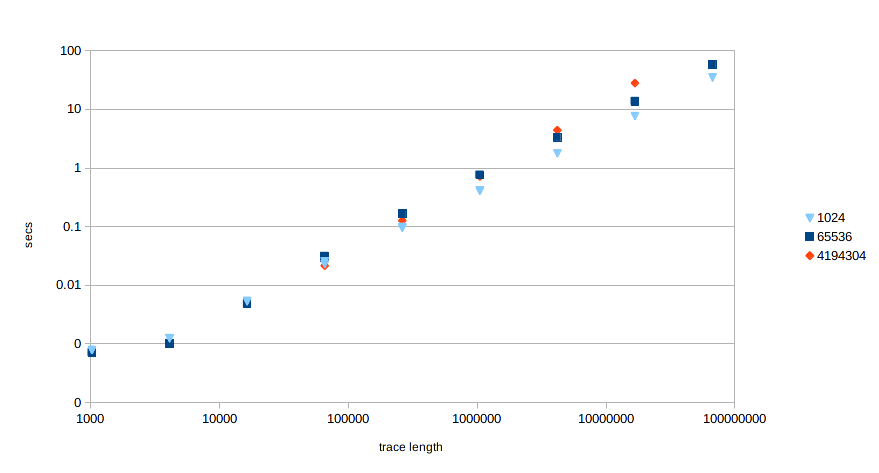
\includegraphics[width=\textwidth]{itree}
\caption{Runtimes in seconds (minimum of 10 runs) of the interval tree algorithm.
Data sets are labelled with the domain size.}
\label{fig:resultsplotitree}
\end{figure}

\begin{figure}
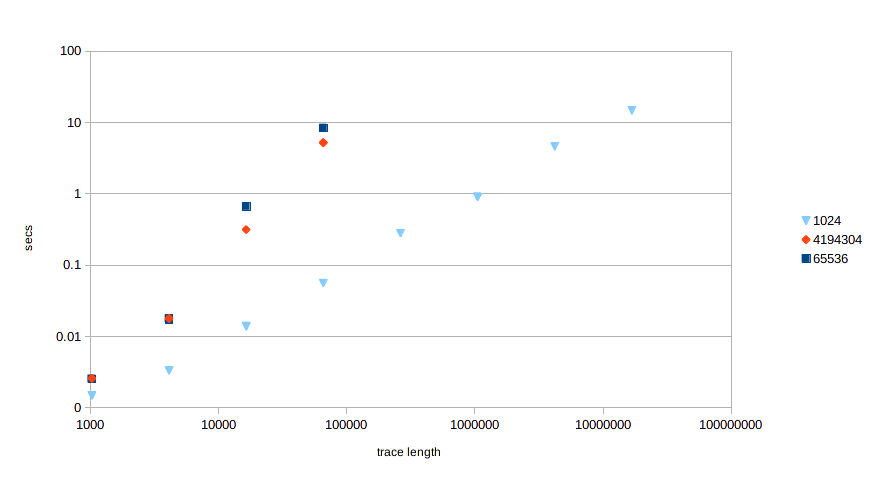
\includegraphics[width=\textwidth]{naive}
\caption{Runtimes in seconds (minimum of 10 runs) of the naive algorithm.
Data sets are labelled with the domain size.}
\label{fig:resultsplotnaive}
\end{figure}

\begin{figure}
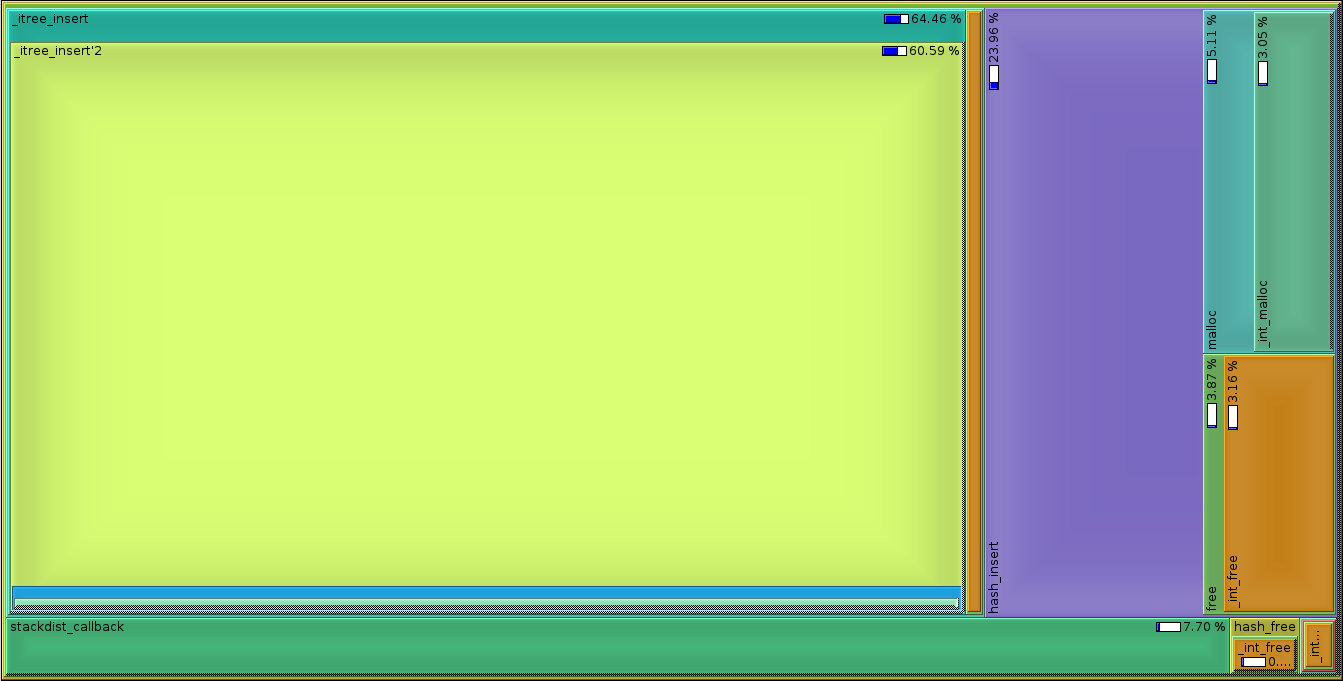
\includegraphics[width=\textwidth]{calleemap}
\caption{The callee map of an lru-misses run with the interval tree algorithm}
\label{fig:calleemap}
\end{figure}

\section{Analysis}

The first point to mention is the effect of compiler optimizations on this application.
We observed a slowdown by a factor of $3$ when \verb|lru-misses| was compiled without the \verb|-O3| flag.
After \verb|-O3|, none of the other optimization attempts we made (branch hints, unrolling loops, inlining
string functions, omitting the frame pointer) had any effect (and a few actually hurt the
performance).

\verb|valgrind| shows us that a large portion (over 35 \%) of the time spent in \verb|hash| was
used for \lstinline|malloc()| and \lstinline|free()|; a good point for
further optimization would be either preallocating the entire hash area, or writing
our own allocator which could use strategies such as doubling the size of allocated
memory when needed.

Generally, the results turned out as expected. For small ($m = 1024$) domains, which can be compared
to programs with good temporal locality characteristics, the naive algorithm performed
very well even for large trace sizes. However, as soon as the domain size was increased,
runtimes went throught the roof. For $n = 262144, m = 1024$, the naive algorithm took around $0.28$ seconds,
but over one minute when the domain was increased to $m = 65536$. It should be noted that the
naive algorithm was comparable to the interval tree implementation for a maximum stack depth of $1024$.

An interesting point was traces with a domain of $2^{22}$ actually caused the naive algorithm
to perform better than traces with a domain of $2^{16}$. We were not able to pinpoint the
cause of this behavior. A guess could be that less time was spent allocating and deallocating
heap memory since the trace elements were rarely found in the existing stack (and thus did
not have to be freed).

The interval tree algorithm on the other hand performed well for every dataset we could throw
at it. Runtimes were well-behaved for all domain sizes (locality behavior). Larger traces 
exhibited noticeable differences  with different domain sizes, but all of them stayed within
acceptable bounds. The only time we actually reached our self-imposed runtime limit of one minute
was with the largest data set and a domain size of $2^{22}$.

As in the original paper, interval tree maintenance took around $65\%$ of the runtime; hash replacements
used $~25\%$, while the remaining $10\%$ were required to track the sums of misses.

\end{document}
